\documentclass[tikz]{standalone}
%\usetikzlibrary{calc}
\usetikzlibrary{shapes,decorations}

\newcommand{\ImageWidth}{11cm}
\usepackage{tikz}
\usetikzlibrary{decorations.pathreplacing,positioning, arrows.meta}

\begin{document}         
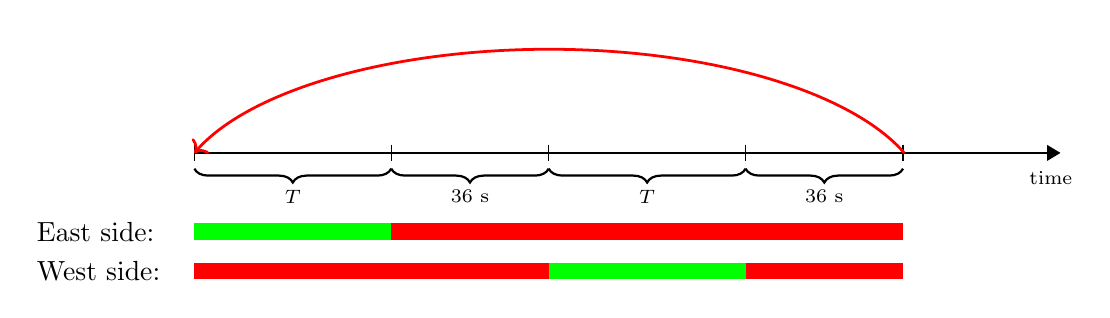
\begin{tikzpicture}
% draw horizontal line   
\draw[thick, -Triangle] (0,0) -- (\ImageWidth,0) node[font=\scriptsize,below left=3pt and -8pt]{time};

% draw vertical lines
\foreach \x in {0,2.5,4.5,7,9}
\draw (\x cm,3pt) -- (\x cm,-3pt);

%\foreach \x/\descr in {1/T,3.5/36s,5.75/T,8/36s}
%\node[font=\scriptsize, text height=3.75ex,
%text depth=.5ex] at (\x,-.3) {$\descr$};


% colored bars east
\draw[green, line width=6pt] 
(0,-1) -- +(2.5,0);
\draw[red, line width=6pt] 
(2.5,-1) -- +(6.5,0);

% colored bars west
\draw[red, line width=6pt] 
(0,-1.5) -- +(4.5,0);
\draw[green, line width=6pt] 
(4.5,-1.5) -- +(2.5,0);
\draw[red, line width=6pt] 
(7,-1.5) -- +(2,0);


\node[text width=3cm] at (-0.5,-1) 
    {East side:};
\node[text width=3cm] at (-0.5,-1.5) 
    {West side:};
    
    
% braces
\draw [thick,decorate,decoration={brace,amplitude=5pt}] (2.5,-.2) -- +(-2.5,0)
       node [black,midway,font=\scriptsize, below=4pt] {$T$};
\draw [thick,decorate,decoration={brace,amplitude=5pt}] (4.5,-.2) -- +(-2,0)
       node [black,midway,font=\scriptsize, below=4pt] {$36$ s};
\draw [thick,decorate,decoration={brace,amplitude=5pt}] (7,-.2) -- +(-2.5,0)
       node [black,midway,font=\scriptsize, below=4pt] {$T$};
\draw [thick,decorate,decoration={brace,amplitude=5pt}] (9,-.2) -- +(-2,0)
       node [black,midway,font=\scriptsize, below=4pt] {$36$ s};
       

% curved line
\draw [<-,red,line width=1pt] (0.0,0.0)  arc
    [
        start angle=160,
        end angle=20,
        x radius=136.5pt,
        y radius = 2cm
    ];       
\end{tikzpicture}

\end{document}